
\documentclass[letter,9pt]{extarticle}

\usepackage[utf8]{inputenc}
\usepackage{concrete}
\usepackage[T1]{fontenc}

\usepackage[none]{hyphenat}
\usepackage{graphicx}
\usepackage{xcolor}
\usepackage{tikz}

\usepackage{amsmath}
\usepackage{amssymb}
\usepackage{amsthm}
\usepackage{textcomp}
\everymath{\displaystyle}
%\usepackage{times}
%\renewcommand\familydefault{\sfdefault}
%\usepackage{tgheros}
%\usepackage[defaultmono,scale=0.85]{droidmono}

\usepackage{multicol}
\setlength{\columnseprule}{0pt}
\setlength{\columnsep}{20.0pt}


\usepackage{geometry}
\geometry{
letterpaper,
total={210mm,297mm},
left=10mm,right=10mm,top=10mm,bottom=15mm}

\linespread{1.3}


% custom title
\makeatletter
\renewcommand*{\maketitle}{%
\noindent
\begin{minipage}{0.4\textwidth}

\begin{tikzpicture}
\node[rectangle,rounded corners=6pt,inner sep=10pt,fill=red!60!yellow,text width= 0.95\textwidth] {\color{white}\Huge \@title};
\end{tikzpicture}
\end{minipage}
\hfill
\begin{minipage}{0.55\textwidth}

\begin{tikzpicture}
\node[rectangle,rounded corners=3pt,inner sep=10pt,draw=red!60!yellow,text width= 0.95\textwidth] {\LARGE Identities};
\end{tikzpicture}
\end{minipage}
\bigskip\bigskip
}%
\makeatother

% custom section
\usepackage[explicit]{titlesec}
\newcommand*\sectionlabel{}
\titleformat{\section}
  {\gdef\sectionlabel{}
   \normalfont\large\bfseries\scshape}
  {\gdef\sectionlabel{\thesection\ }}{0pt}
  {
\noindent
\begin{tikzpicture}
\node[rectangle,rounded corners=3pt,inner sep=4pt,fill=red!60!yellow,text width= 0.95\columnwidth] {\color{white}\sectionlabel#1};
\end{tikzpicture}
  }
\titlespacing*{\section}{2pt}{11pt}{2pt}


% custom footer
\usepackage{lastpage}
\usepackage{fancyhdr}
\makeatletter
\pagestyle{fancy}
\fancyhead{}
\fancyfoot[C]{\footnotesize\ \copyright\ \@date\ \ \@author}
\renewcommand{\headrulewidth}{0pt}
\renewcommand{\footrulewidth}{0pt}
\rfoot{Page \thepage/\pageref{LastPage}}
\makeatother


\title{Trigonometry \\ \ \ \ \ \ \ \ \ \ \ \ \ Reference Sheet}
\author{K. M. Short}
\date{2017}



\begin{document}

\maketitle

\begin{multicols*}{2}


\section*{Remembering the Value Table}

The 
\begin{tabular}{lll}
$a^n a^m = a^{n+m}$ & $\frac{a^n}{a^m} = a^{n-m}$ & $(a^n)^m = a^{n \cdot m}$\\
$a^n a^m = a^{n+m}$ & $\frac{a^n}{a^m} = a^{n-m}$ & $(a^n)^m = a^{n \cdot m}$\\
$a^n a^m = a^{n+m}$ & $\frac{a^n}{a^m} = a^{n-m}$ & $(a^n)^m = a^{n \cdot m}$\\
$a^n a^m = a^{n+m}$ & $\frac{a^n}{a^m} = a^{n-m}$ & $(a^n)^m = a^{n \cdot m}$\\
$a^n a^m = a^{n+m}$ & $\frac{a^n}{a^m} = a^{n-m}$ & $(a^n)^m = a^{n \cdot m}$\\
$a^n a^m = a^{n+m}$ & $\frac{a^n}{a^m} = a^{n-m}$ & $(a^n)^m = a^{n \cdot m}$
\end{tabular}


\section{The Real Equations}

The only real equations of the six you are used to seeing are the ones you need to worry about, they are $\sin$ and $\cos$.

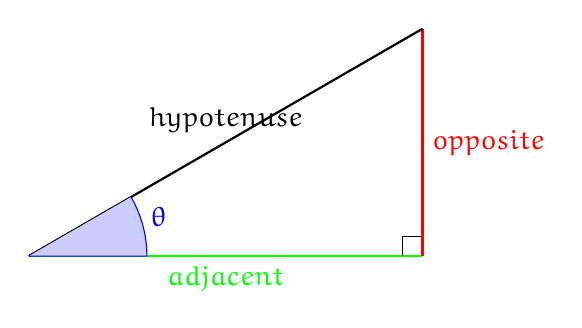
\begin{tikzpicture}[scale=5]
\draw[thick,color=green] (0,0) -- node[below] {$adjacent$} (1,0);
\draw[thick,color=red] (1,0) -- node[right] {$opposite$} (1,0.57735);
\draw[thick,color=black] (1,0.57735) -- node[above] {$hypotenuse$} (0,0);
\filldraw[fill=blue!20!white,draw=blue] (0,0) -- (0.3,0) arc (0:30:0.3); 
\node[color=blue] at (0.33,0.1) {$\theta$};
\draw (0.95,0) -- (0.95,0.05) -- (1,0.05);
\end{tikzpicture}

\medskip

\begin{tabular}{ll}
$\sin\theta = \frac{opposite}{hypotenuse}$ & $\cos\theta = \frac{adjacent}{hypotenuse}$ \\[1ex]
\end{tabular}

\section{The Other Basic Equations}
These are all simply short hand for the above $\sin$ and $\cos$


\begin{tabular}{ll}
$\tan\theta = \frac{opposite}{adjacent}$ & $\cot\theta = \frac{adjacent}{opposite}$ \\[2ex]
$\sec\theta = \frac{hypotenuse}{adjacent}$ & $\csc\theta = \frac{hypotenuse}{opposite}$\\[1ex]
\end{tabular}

\section{Trigonometry}

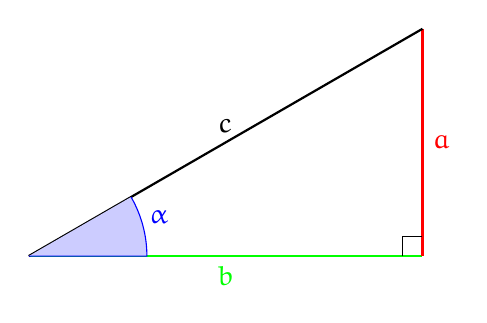
\begin{tikzpicture}[scale=5]
\draw[thick,color=green] (0,0) -- node[below] {$b$} (1,0);
\draw[thick,color=red] (1,0) -- node[right] {$a$} (1,0.57735);
\draw[thick,color=black] (1,0.57735) -- node[above] {$c$} (0,0);
\filldraw[fill=blue!20!white,draw=blue] (0,0) -- (0.3,0) arc (0:30:0.3); 
\node[color=blue] at (0.33,0.1) {$\alpha$};
\draw (0.95,0) -- (0.95,0.05) -- (1,0.05);
\end{tikzpicture}

\medskip

\begin{tabular}{ll}
$\sin\alpha = \frac{a}{c}$ & $\cos\alpha = \frac{b}{c}$ \\[1ex]
$\tan\alpha = \frac{a}{b}$ & $\cot\alpha = \frac{b}{a}$ \\
\end{tabular}


\section{Algebra}

\begin{tabular}{lll}
$a^n a^m = a^{n+m}$ & $\frac{a^n}{a^m} = a^{n-m}$ & $(a^n)^m = a^{n \cdot m}$\\
$a^n a^m = a^{n+m}$ & $\frac{a^n}{a^m} = a^{n-m}$ & $(a^n)^m = a^{n \cdot m}$\\
$a^n a^m = a^{n+m}$ & $\frac{a^n}{a^m} = a^{n-m}$ & $(a^n)^m = a^{n \cdot m}$\\
$a^n a^m = a^{n+m}$ & $\frac{a^n}{a^m} = a^{n-m}$ & $(a^n)^m = a^{n \cdot m}$\\
$a^n a^m = a^{n+m}$ & $\frac{a^n}{a^m} = a^{n-m}$ & $(a^n)^m = a^{n \cdot m}$\\
$a^n a^m = a^{n+m}$ & $\frac{a^n}{a^m} = a^{n-m}$ & $(a^n)^m = a^{n \cdot m}$
\end{tabular}


\section{Trigonometry}

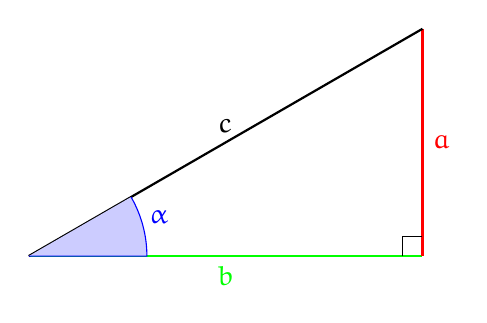
\begin{tikzpicture}[scale=5]
\draw[thick,color=green] (0,0) -- node[below] {$b$} (1,0);
\draw[thick,color=red] (1,0) -- node[right] {$a$} (1,0.57735);
\draw[thick,color=black] (1,0.57735) -- node[above] {$c$} (0,0);
\filldraw[fill=blue!20!white,draw=blue] (0,0) -- (0.3,0) arc (0:30:0.3); 
\node[color=blue] at (0.33,0.1) {$\alpha$};
\draw (0.95,0) -- (0.95,0.05) -- (1,0.05);
\end{tikzpicture}

\medskip

\begin{tabular}{ll}
$\sin\alpha = \frac{a}{c}$ & $\cos\alpha = \frac{b}{c}$ \\[1ex]
$\tan\alpha = \frac{a}{b}$ & $\cot\alpha = \frac{b}{a}$ \\
\end{tabular}


\section{The End}

Lorem ipsum dolor sit amet, consectetur adipiscing elit, sed do eiusmod tempor incididunt ut labore et dolore magna aliqua. Ut enim ad minim veniam, quis nostrud exercitation ullamco laboris nisi ut aliquip ex ea commodo consequat. Duis aute irure dolor in reprehenderit in voluptate velit esse cillum dolore eu fugiat nulla pariatur. Excepteur sint occaecat cupidatat non proident, sunt in culpa qui officia deserunt mollit anim id est laborum.


\end{multicols*}

\end{document}
